%%%%%%%%%%%%%%%%
%% Preambule  %%
%%%%%%%%%%%%%%%%

\documentclass[11pt]{article}

\usepackage{amsmath,amsfonts,amssymb}
\usepackage{upgreek}
\usepackage{enumerate}
\usepackage{enumitem}
\usepackage{multicol}
\usepackage{scrextend}

\usepackage[all]{xy}
\usepackage{tikz-qtree}
\usepackage[margin=2.5cm]{geometry}

\usepackage{fancyhdr}
\usepackage{lastpage}
\usepackage{subcaption}

\setlength{\parindent}{0pt}

\pagestyle{fancy}

\lhead{\opdrachtNaam\ \opdrachtNummer}
\rhead{\naam(\studentNummer)}
\rfoot{Page\ \thepage\ of\ \pageref{LastPage}}
\lfoot{\datum}
\cfoot{}

\renewcommand\headrulewidth{0.4pt}
\renewcommand\footrulewidth{0.4pt}

\newcommand{\E}{\exists}
\newcommand{\A}{\forall}


\newcommand{\ccen}[2]{\llap{$#1$}${}\mathrel{\circ}{}$\rlap{$#2$}}


%%%%%%%%%%%%%%
%% Gegevens %%
%%%%%%%%%%%%%%

\newcommand{\naam}          {Stefan Schenk}
\newcommand{\studentNummer} {11881798}
\newcommand{\opdrachtNaam}  {Assignment}
\newcommand{\opdrachtNummer}{1}
\newcommand{\datum}         {November 2017}


%%%%%%%%%%%%%%%%
%% Antwoorden %%
%%%%%%%%%%%%%%%%

\begin{document}


%%%%%%%%%%%%%%%%
%% Question 1 %%
%%%%%%%%%%%%%%%%

\section*{Question 1}

\begin{enumerate}[label=(\alph*)]

  \item \textit{Produce clear images for the surface plots for both Model CT
  and Model D, and provide screenshots for the input membership functions as
  well as the output membership functions. State your answers clearly for each
  model, separately.}

  \begin{figure}[ht!]
  \centering
  \begin{subfigure}{.5\textwidth}
    \centering
    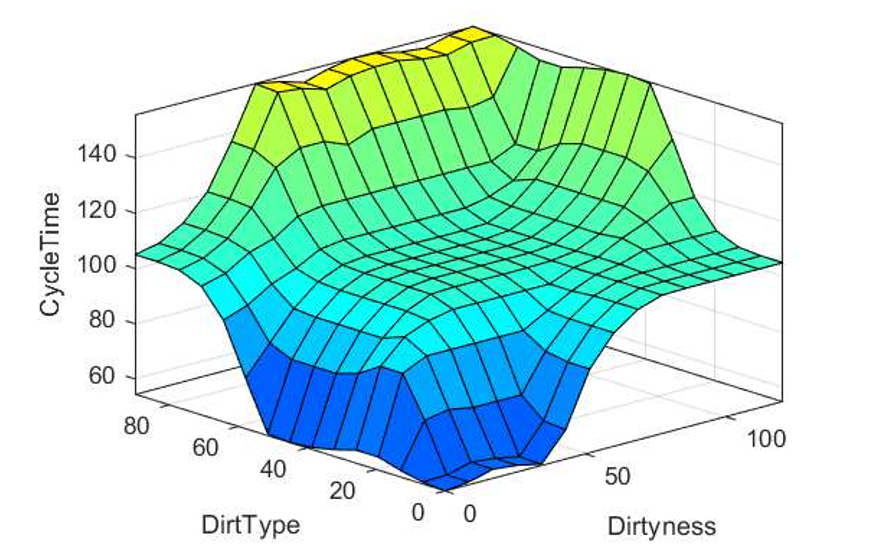
\includegraphics[width=.9\linewidth]{res/image1}
    \caption{ModelCT}
    \label{fig:sub1}
  \end{subfigure}%
  \begin{subfigure}{.5\textwidth}
    \centering
    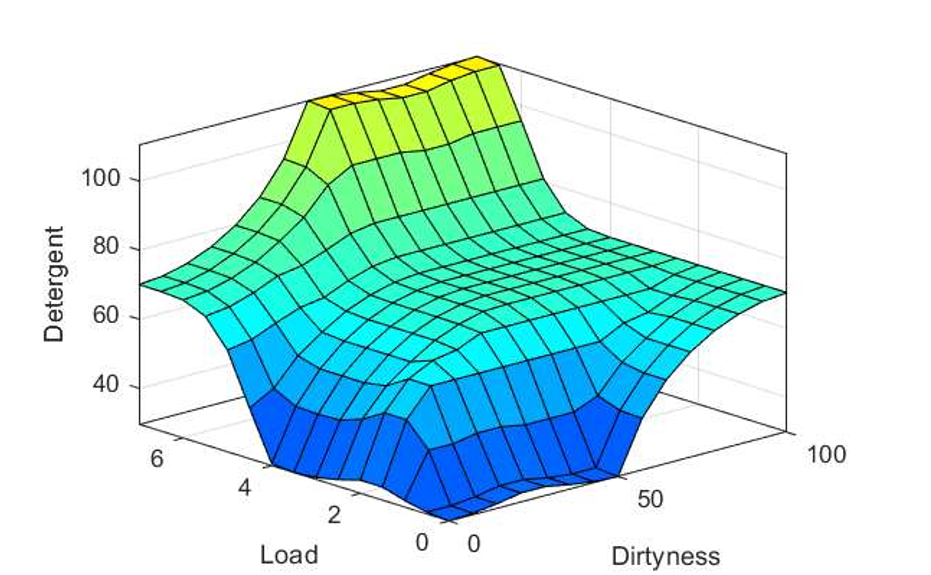
\includegraphics[width=.9\linewidth]{res/image2}
    \caption{ModelD}
    \label{fig:sub2}
  \end{subfigure}
  \end{figure}

  \begin{figure}[ht!]
  \centering
  \begin{subfigure}{.5\textwidth}
    \centering
    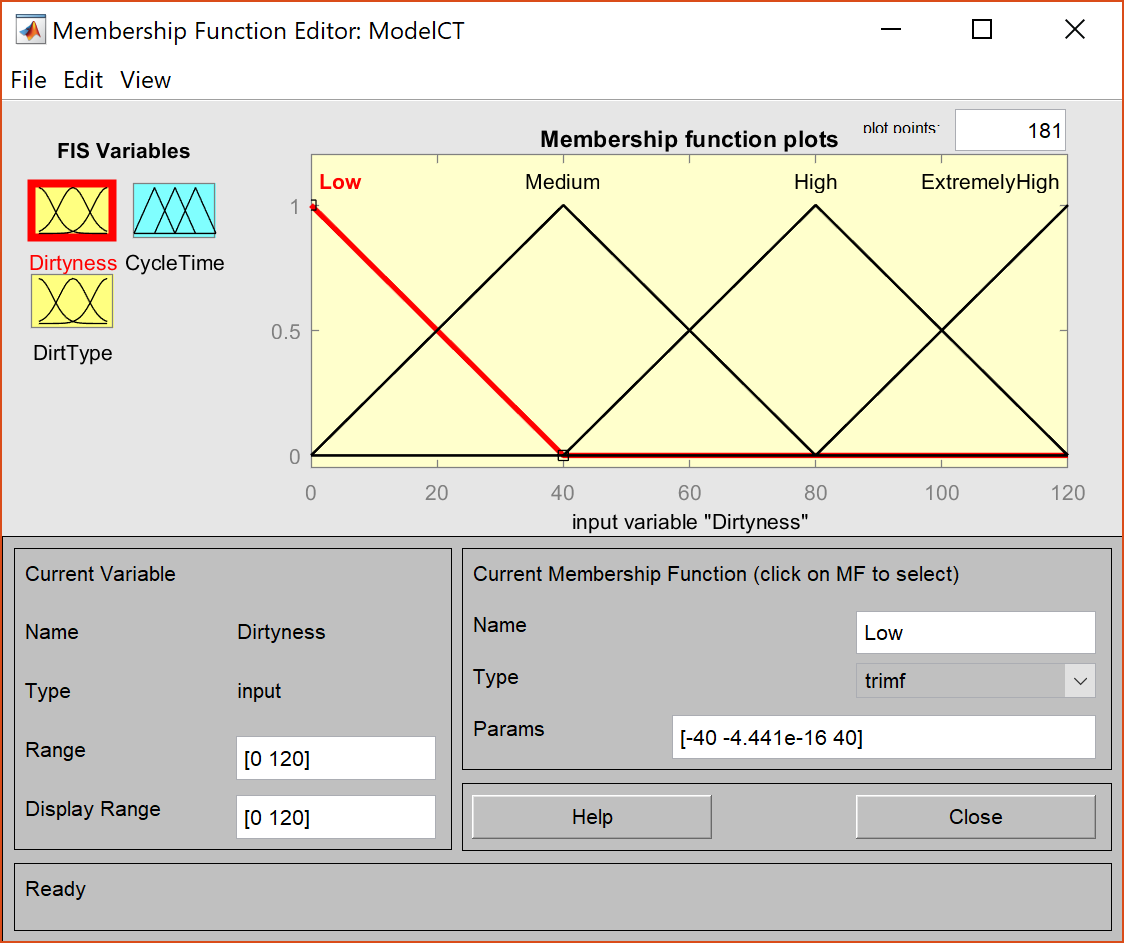
\includegraphics[width=.9\linewidth]{res/image1_dirtyness}
    \caption{ModelCT - Dirtyness Input}
    \label{fig:sub1}
  \end{subfigure}%
  \begin{subfigure}{.5\textwidth}
    \centering
    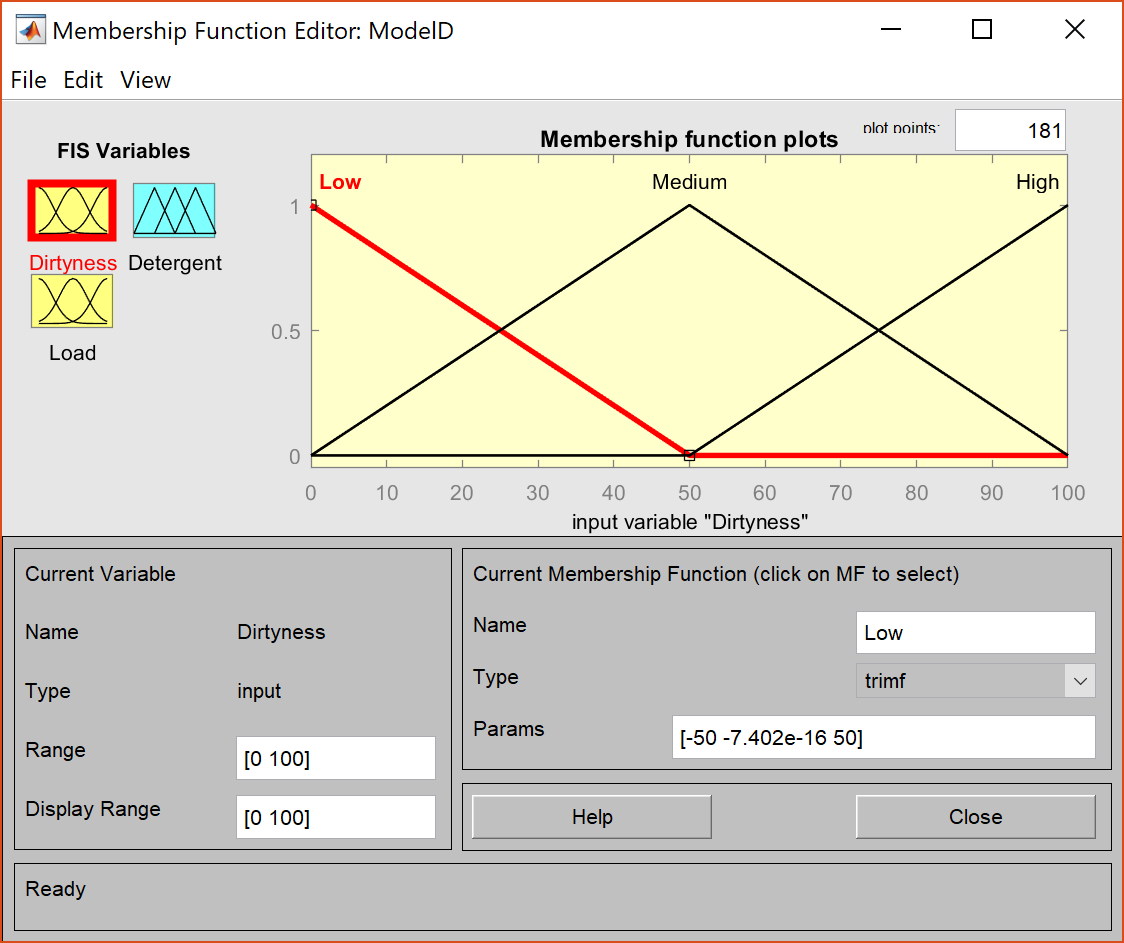
\includegraphics[width=.9\linewidth]{res/image2_dirtyness}
    \caption{ModelD - Dirtyness Input}
    \label{fig:sub2}
  \end{subfigure}
  \end{figure}

  \begin{figure}[ht!]
  \centering
  \begin{subfigure}{.5\textwidth}
    \centering
    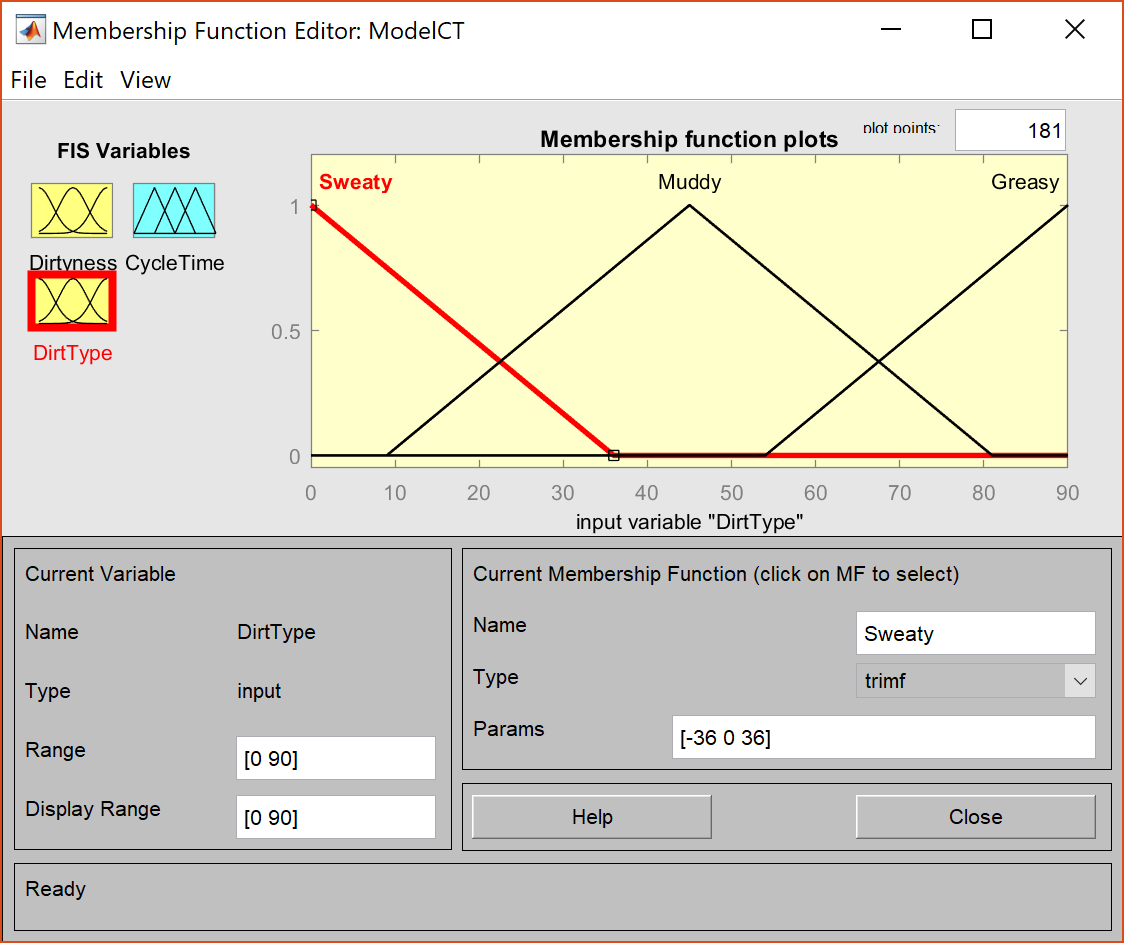
\includegraphics[width=.9\linewidth]{res/image1_dirttype}
    \caption{ModelCT - DirtType Input}
    \label{fig:sub1}
  \end{subfigure}%
  \begin{subfigure}{.5\textwidth}
    \centering
    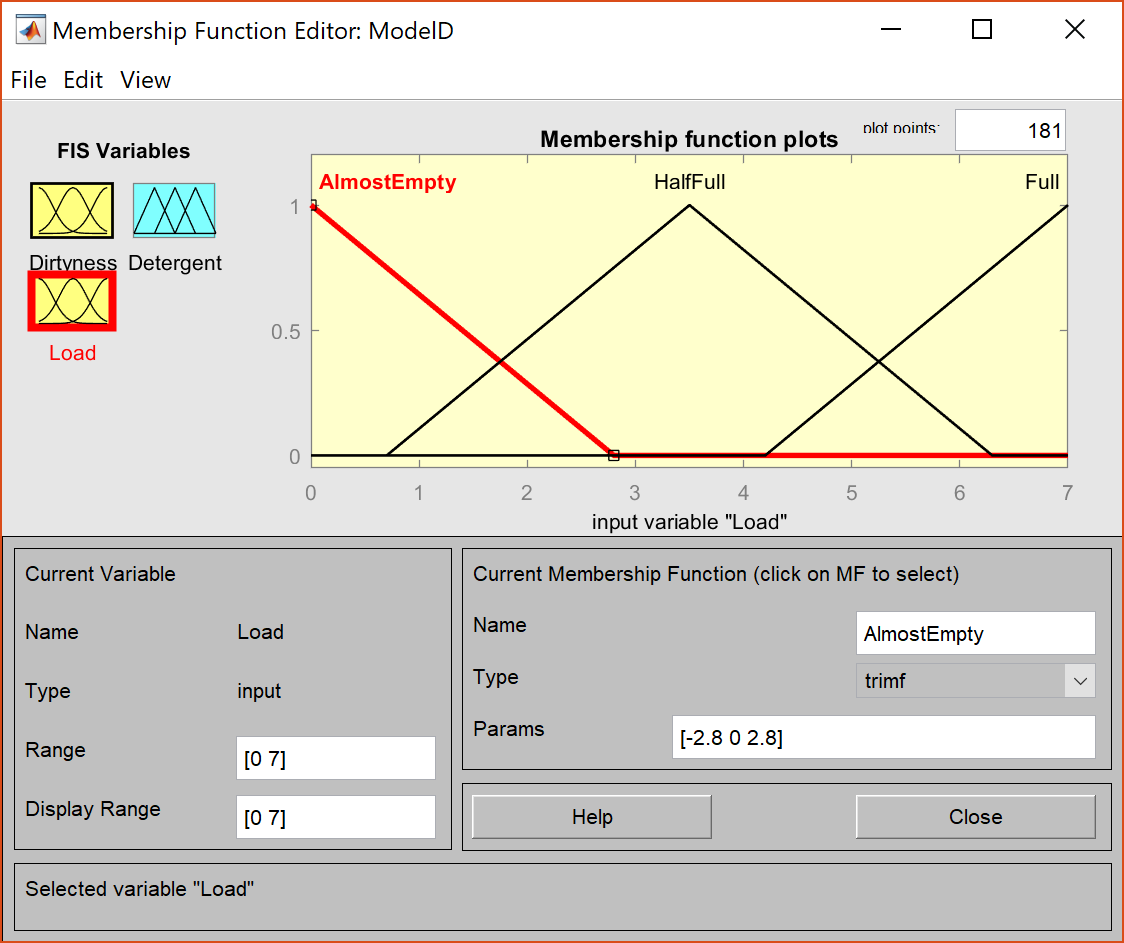
\includegraphics[width=.9\linewidth]{res/image2_load}
    \caption{ModelD - Load Input}
    \label{fig:sub2}
  \end{subfigure}
  \end{figure}

  \begin{figure}[ht!]
  \centering
  \begin{subfigure}{.5\textwidth}
    \centering
    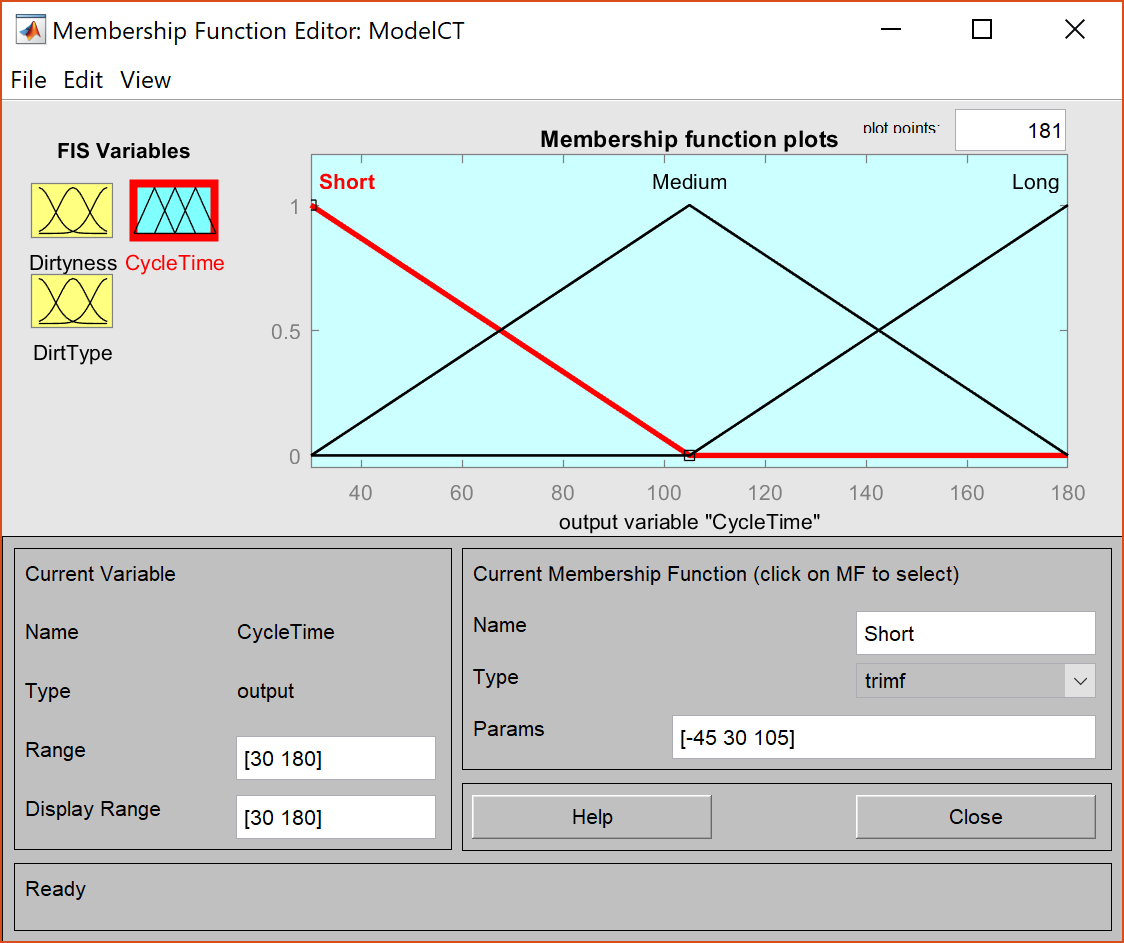
\includegraphics[width=.9\linewidth]{res/image1_cycletime}
    \caption{ModelCT - CycleTime Output}
    \label{fig:sub1}
  \end{subfigure}%
  \begin{subfigure}{.5\textwidth}
    \centering
    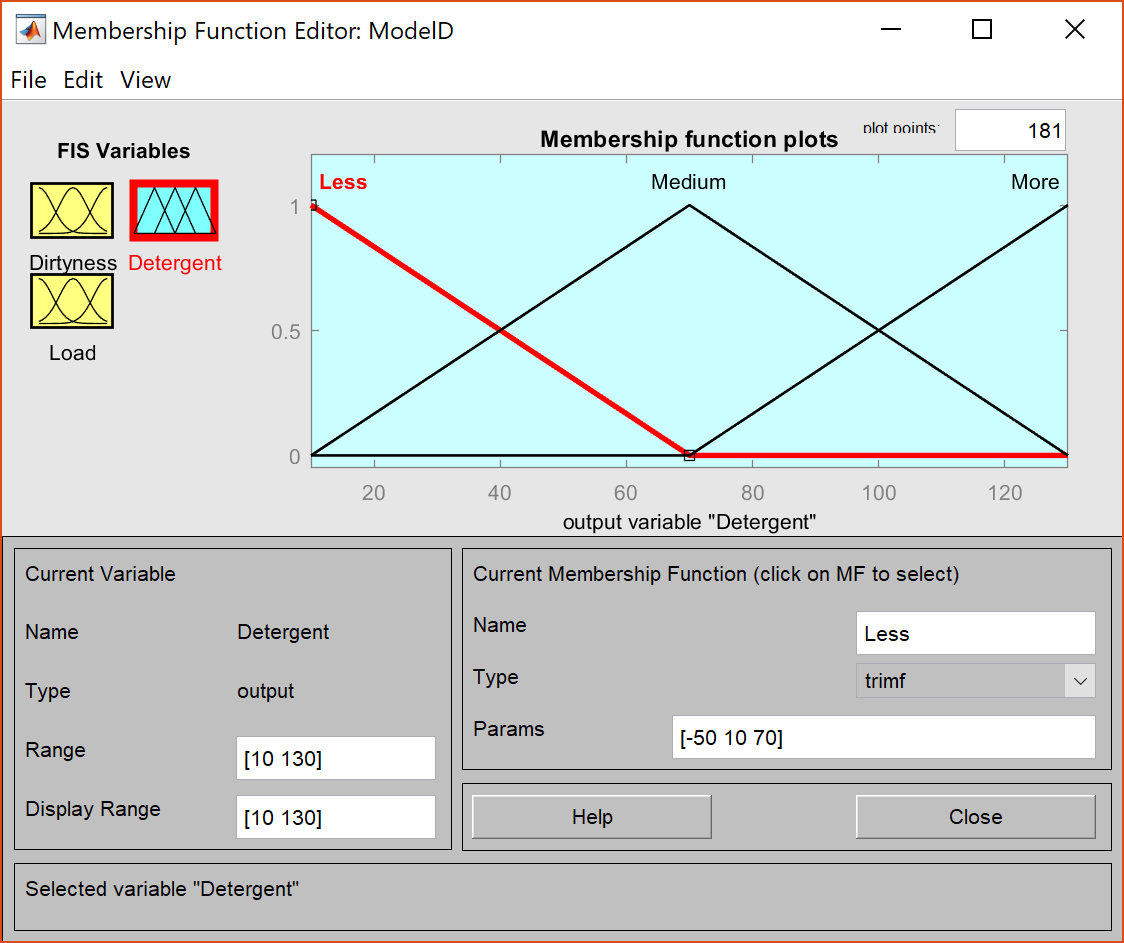
\includegraphics[width=.9\linewidth]{res/image2_detergent}
    \caption{ModelD - Detergent Output}
    \label{fig:sub2}
  \end{subfigure}
  \end{figure}

  \pagebreak

  \item \textit{Modify the rule bases for both Model CT and Model D by reducing
  as much rules as possible, without changing the behaviour of the system too
  much. How would you explain the behaviour change while logically maintaining
  the rule base? If this is possible, give an example of your reasoning. Report
  the new rule bases, separately, and justify your decisions by briefly
  describing your motivation.}

  By ticking the not box, it is possible to avoid make rules seperately for each
  non-changing variable, reducing the number of rules from 9 to 6 for ModelD,
  and from 12 to 10 for ModelCT.

  \subsection*{ModelD}

  Before:
  \begin{enumerate}[label=(\arabic*)]
    \item If (Dirtyness is Low) and (Load is AlmostEmpty) then (Detergent is
    Less) (1)
    \item If (Dirtyness is Medium) and (Load is AlmostEmpty) then (Detergent is
    Less) (1)
    \item If (Dirtyness is High) and (Load is AlmostEmpty) then (Detergent is
    Medium) (1)
    \item If (Dirtyness is Low) and (Load is HalfFull) then (Detergent is Less)
    (1)
    \item If (Dirtyness is Medium) and (Load is HalfFull) then (Detergent is
    Medium) (1)
    \item If (Dirtyness is High) and (Load is HalfFull) then (Detergent is
    Medium) (1)
    \item If (Dirtyness is Low) and (Load is Full) then (Detergent is Medium)
    (1)
    \item If (Dirtyness is Medium) and (Load is Full) then (Detergent is More)
    (1)
    \item If (Dirtyness is High) and (Load is Full) then (Detergent is More) (1)
  \end{enumerate}

  After:
  \begin{enumerate}[label=(\arabic*)]
    \item If (Dirtyness is not High) and (Load is AlmostEmpty) then (Detergent
    is Less) (1)
    \item If (Dirtyness is High) and (Load is AlmostEmpty) then (Detergent is
    Medium) (1)
    \item If (Dirtyness is Low) and (Load is HalfFull) then (Detergent is Less)
    (1)
    \item If (Dirtyness is not Low) and (Load is HalfFull) then (Detergent
    is Medium) (1)
    \item If (Dirtyness is Low) and (Load is Full) then (Detergent is Medium)
    (1)
    \item If (Dirtyness is not Low) and (Load is Full) then (Detergent is More)
    (1)
  \end{enumerate}

  \subsection*{ModelCT}

  Before:
  \begin{enumerate}[label=(\arabic*)]
    \item If (Dirtyness is Low) and (DirtType is Sweaty) then (CycleTime is
    Short) (1)
    \item If (Dirtyness is Medium) and (DirtType is Sweaty) then (CycleTime is
    Short) (1)
    \item If (Dirtyness is High) and (DirtType is Sweaty) then (CycleTime is
    Medium) (1)
    \item If (Dirtyness is ExtremelyHigh) and (DirtType is Sweaty) then
    (CycleTime is Medium) (1)
    \item If (Dirtyness is Low) and (DirtType is Muddy) then (CycleTime is
    Short) (1)
    \item If (Dirtyness is Medium) and (DirtType is Muddy) then (CycleTime is
    Medium) (1)
    \item If (Dirtyness is High) and (DirtType is Muddy) then (CycleTime is
    Medium) (1)
    \item If (Dirtyness is ExtremelyHigh) and (DirtType is Muddy) then
    (CycleTime is Long) (1)
    \item If (Dirtyness is Low) and (DirtType is Greasy) then (CycleTime is
    Medium) (1)
    \item If (Dirtyness is Medium) and (DirtType is Greasy) then (CycleTime is
    Long) (1)
    \item If (Dirtyness is High) and (DirtType is Greasy) then (CycleTime is
    Long) (1)
    \item If (Dirtyness is ExtremelyHigh) and (DirtType is Greasy) then
    (CycleTime is Long) (1)
  \end{enumerate}

  After:
  \begin{enumerate}[label=(\arabic*)]
    \item If (Dirtyness is Low) and (DirtType is Sweaty) then (CycleTime is
    Short) (1)
    \item If (Dirtyness is Medium) and (DirtType is Sweaty) then (CycleTime is
    Short) (1)
    \item If (Dirtyness is High) and (DirtType is Sweaty) then (CycleTime is
    Medium) (1)
    \item If (Dirtyness is ExtremelyHigh) and (DirtType is Sweaty) then
    (CycleTime is Medium) (1)
    \item If (Dirtyness is Low) and (DirtType is Muddy) then (CycleTime is
    Short) (1)
    \item If (Dirtyness is Medium) and (DirtType is Muddy) then
    (CycleTime is Medium) (1)
    \item If (Dirtyness is High) and (DirtType is Muddy) then (CycleTime is
    Medium) (1)
    \item If (Dirtyness is ExtremelyHigh) and (DirtType is Muddy) then
    (CycleTime is Long) (1)
    \item If (Dirtyness is Low) and (DirtType is Greasy) then (CycleTime is
    Medium) (1)
    \item If (Dirtyness is not Low) and (DirtType is Greasy) then (CycleTime is
    Long) (1)
  \end{enumerate}

  \item \textit{What kind of inference system did you implement for Model CT?
  Explain your answer by giving reason.}

  A Mamdani-type rule based inference system. The consequents are represented
  as fuzzy sets, the aggregation is performed on output fuzzy sets by taking the
  union.

  \item \textit{Try decreasing and increasing the overlap between both the input and output fuzzy sets for Model D. How does this influence the behaviour of the system? Explain briefly.}

  Increasing overlap makes the surface of the modal look more flat. Decreasing
  overlap decreases the complexity of the surface.

  \begin{figure}[ht!]
  \centering
  \begin{subfigure}{.5\textwidth}
    \centering
    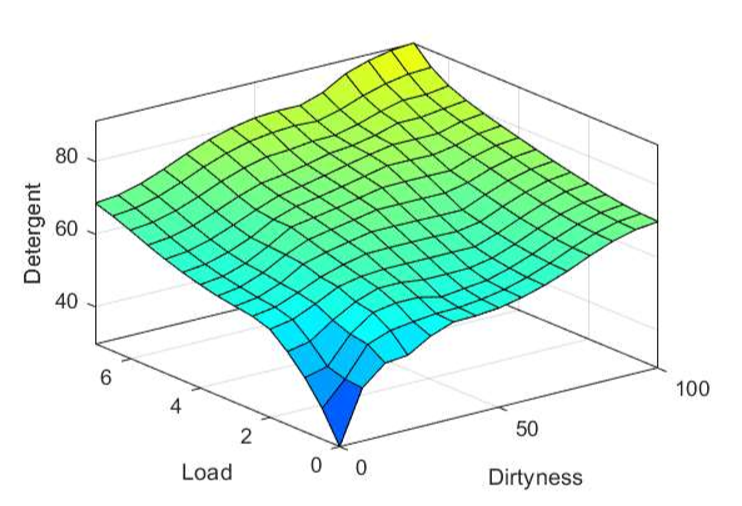
\includegraphics[width=.9\linewidth]{res/modelD_flat}
    \caption{ModelD - Increased Overlap}
    \label{fig:sub1}
  \end{subfigure}%
  \begin{subfigure}{.5\textwidth}
    \centering
    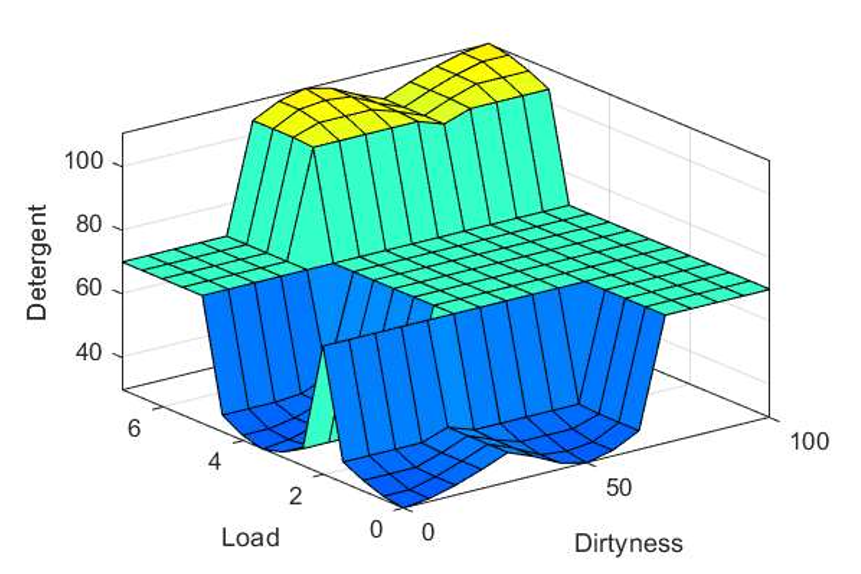
\includegraphics[width=.9\linewidth]{res/modelD_complex}
    \caption{ModelD - Decreased Overlap}
    \label{fig:sub2}
  \end{subfigure}
\end{figure}

  \pagebreak

  \item \textit{Change the settings according to the following parameters one
  at a time. How does this influence the behaviour of the system? Explain the
  meaning of the setting and describe your observations briefly. After each
  change, go back to the default settings.}

  \begin{enumerate}[label=(\roman*)]

    \item Aggregation = sum:

    \begin{figure}[ht!]
    \centering
    \begin{subfigure}{.5\textwidth}
      \centering
      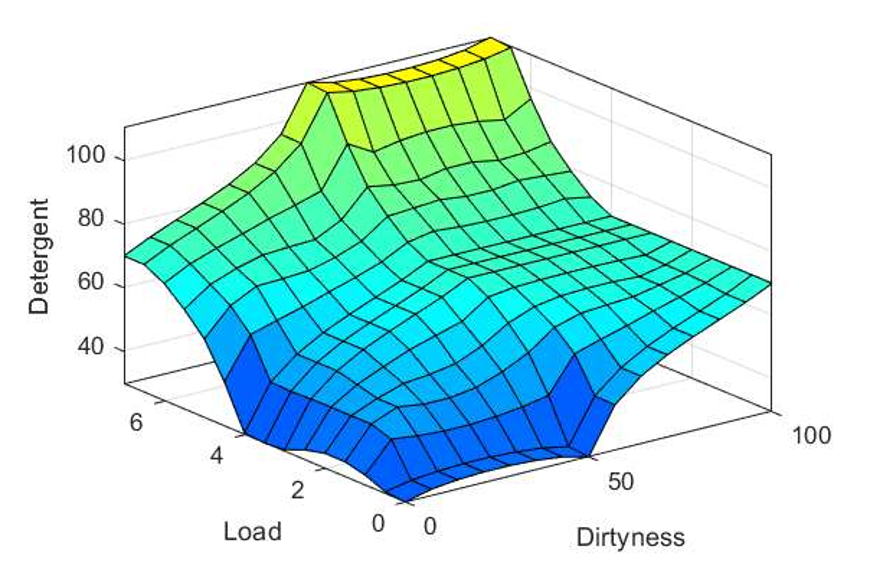
\includegraphics[width=.9\linewidth]{res/modelD_aggregation}
      \caption{ModelD - Aggregation = sum}
      \label{fig:sub1}
    \end{subfigure}%
    \begin{subfigure}{.5\textwidth}
      \centering
      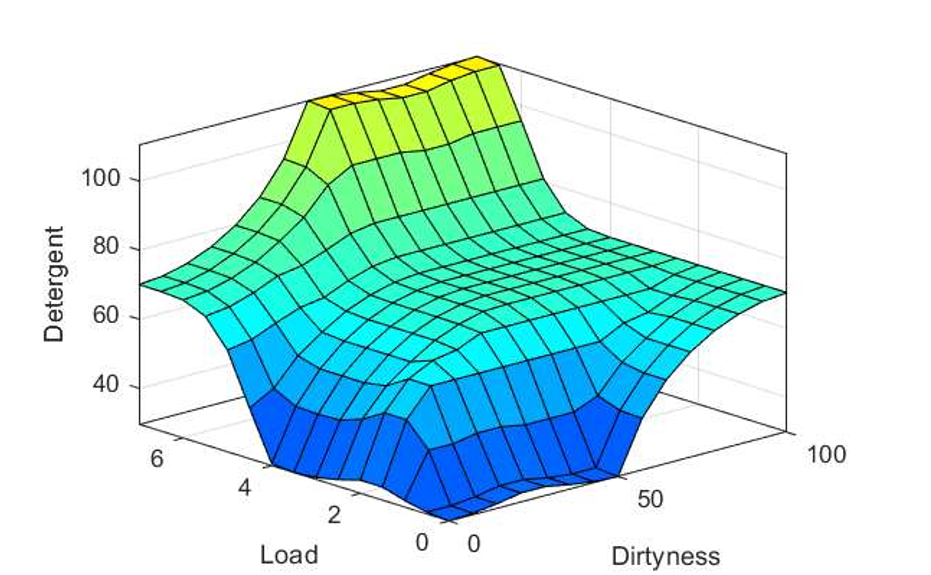
\includegraphics[width=.9\linewidth]{res/image2}
      \caption{ModelD - Original}
      \label{fig:sub2}
    \end{subfigure}
    \end{figure}

    \item Defuzzification = bisector:

    \begin{figure}[ht!]
    \centering
    \begin{subfigure}{.5\textwidth}
      \centering
      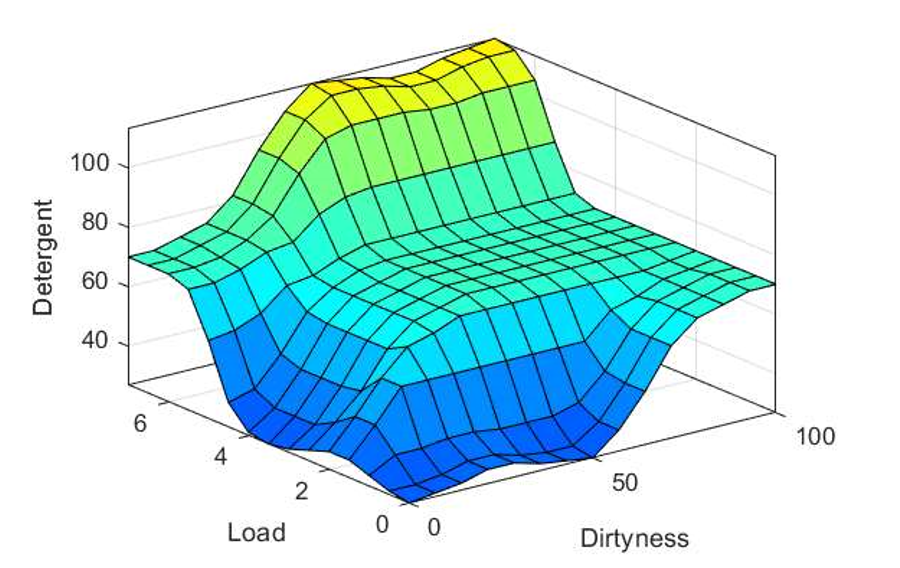
\includegraphics[width=.9\linewidth]{res/modelD_bisector}
      \caption{ModelD - Defuzzification = bisector}
      \label{fig:sub1}
    \end{subfigure}%
    \begin{subfigure}{.5\textwidth}
      \centering
      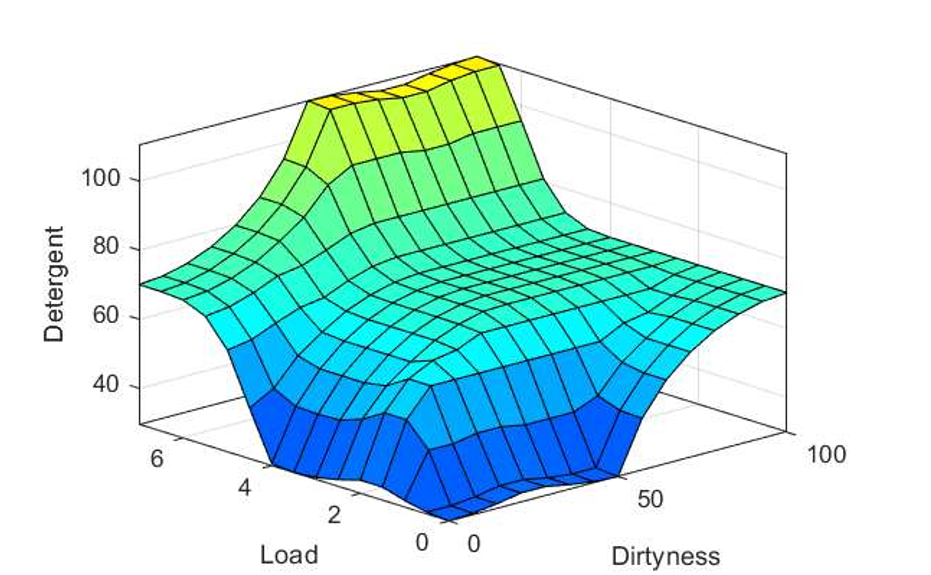
\includegraphics[width=.9\linewidth]{res/image2}
      \caption{ModelD - Original}
      \label{fig:sub2}
    \end{subfigure}
    \end{figure}

    \item Defuzzification = SoM:

    \begin{figure}[ht!]
    \centering
    \begin{subfigure}{.5\textwidth}
      \centering
      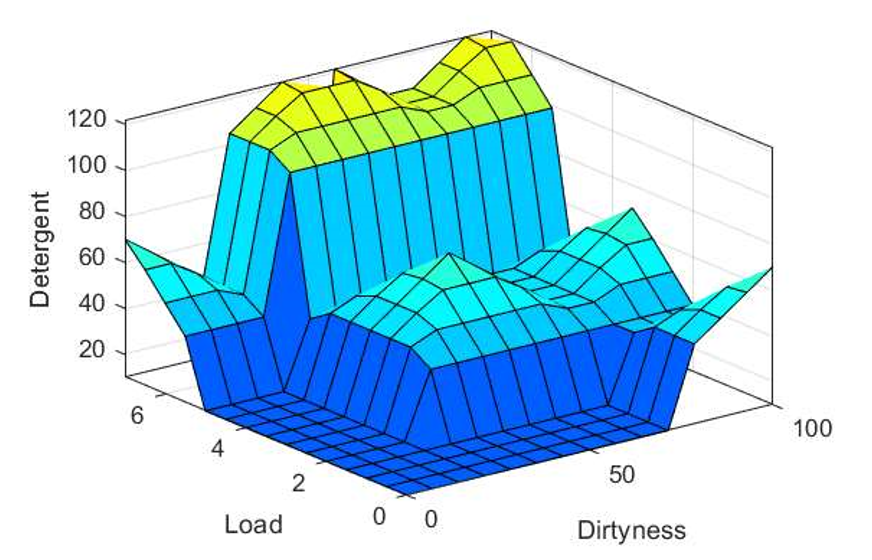
\includegraphics[width=.9\linewidth]{res/modelD_som}
      \caption{ModelD - Defuzzification = som}
      \label{fig:sub1}
    \end{subfigure}%
    \begin{subfigure}{.5\textwidth}
      \centering
      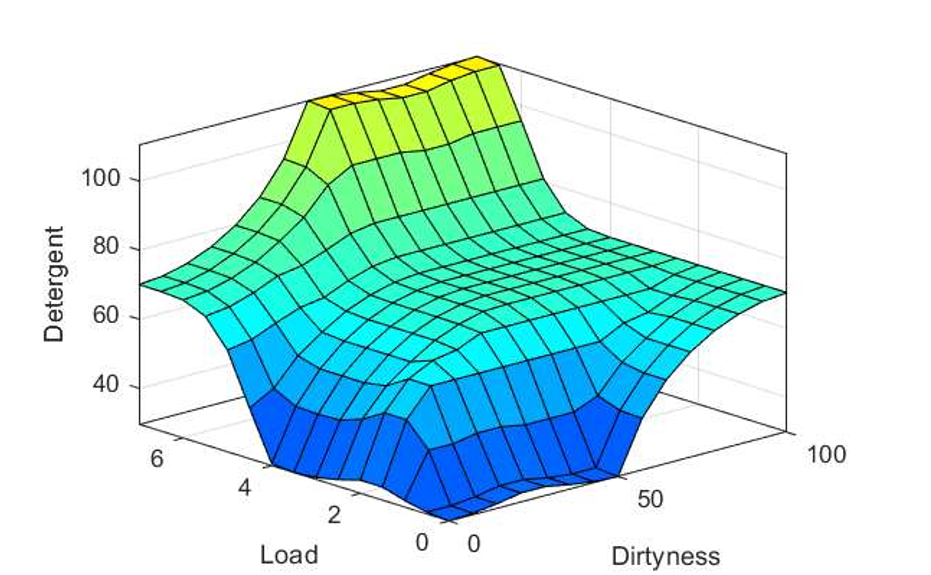
\includegraphics[width=.9\linewidth]{res/image2}
      \caption{ModelD - Original}
      \label{fig:sub2}
    \end{subfigure}
    \end{figure}

    \pagebreak

    \item T-norm = prod:

    \begin{figure}[ht!]
    \centering
    \begin{subfigure}{.5\textwidth}
      \centering
      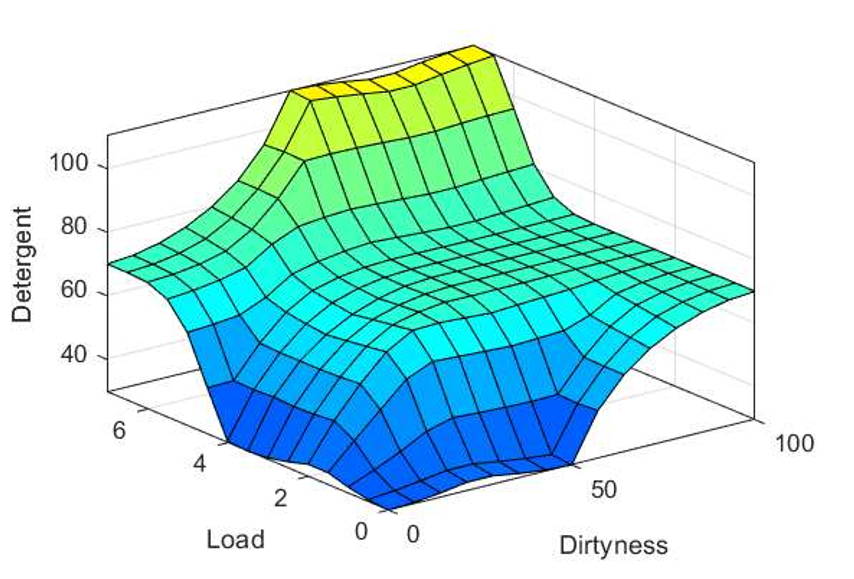
\includegraphics[width=.9\linewidth]{res/modelD_t-norm}
      \caption{ModelD - T-norm = prod}
      \label{fig:sub1}
    \end{subfigure}%
    \begin{subfigure}{.5\textwidth}
      \centering
      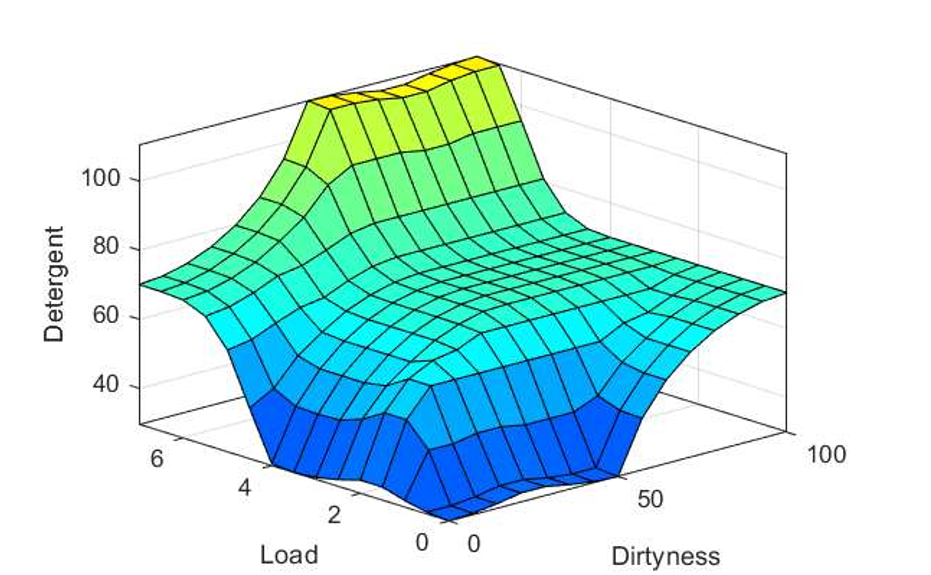
\includegraphics[width=.9\linewidth]{res/image2}
      \caption{ModelD - Original}
      \label{fig:sub2}
    \end{subfigure}
    \end{figure}

  \end{enumerate}


  \item \textit{Change the input membership functions to be Gaussian rather than
  triangular for both inputs of Model CT. How does this influence the behaviour
  of the system? Explain briefly.}

  The membership level of an input variable that lies further away from the
  linguistic term is decreasing slowly at first, but the further it moves away,
  the faster it decreases, opposed to the immediate linear drop of membership.

  \begin{figure}[ht!]
  \centering
  \begin{subfigure}{.5\textwidth}
    \centering
    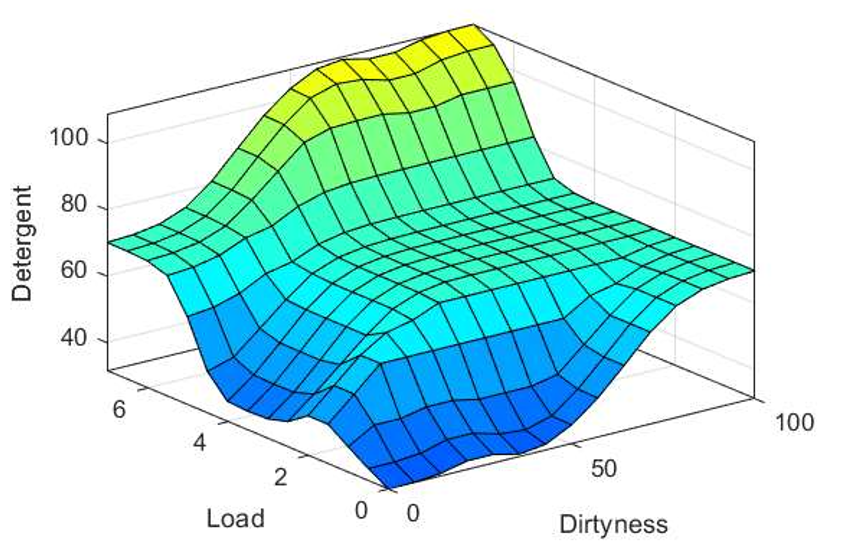
\includegraphics[width=.9\linewidth]{res/modelD_gaussian}
    \caption{ModelD - MF = gaussian}
    \label{fig:sub1}
  \end{subfigure}%
  \begin{subfigure}{.5\textwidth}
    \centering
    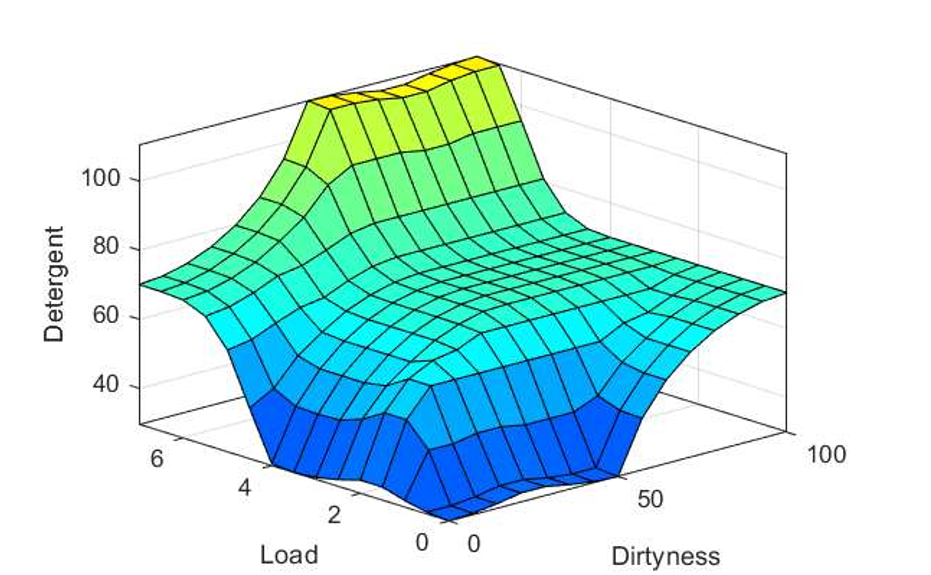
\includegraphics[width=.9\linewidth]{res/image2}
    \caption{ModelD - Original}
    \label{fig:sub2}
  \end{subfigure}
  \end{figure}

\end{enumerate}


%%%%%%%%%%%%%%%%
%% Question 2 %%
%%%%%%%%%%%%%%%%

\pagebreak

\section*{Question 2}

So, my manager realised that none of the models (D and CT) are good fit to solve
the customers' complaints. Implying that all the complaints are still unsolved.
It can be assumed that the complaints are still in effect because the
two systems aren't used simultaniously. So either the long cycle time is
resolved, or the amount of detergent is resolved.

This implies that merging the two models into FoFL would already solve the
majority of the problems. Therefore, merging the two models, D and CT into a
hierarchical FLS would solve the problems with minimal effort. Instead we
design a totally new system FoFL.

\begin{enumerate}[label=(\alph*)]

  \item \textit{Show the input and output membership functions and the surfaces
  of your final (most preferred) system for the following 2 inputs - 1 output
  combinations: [Dirtiness, DirtType, CycleTime], [Load, Dirtiness, CycleTime]
  and [Load, DirtType, Detergent].}

  \begin{figure}[ht!]
  \centering
  \begin{subfigure}{.5\textwidth}
    \centering
    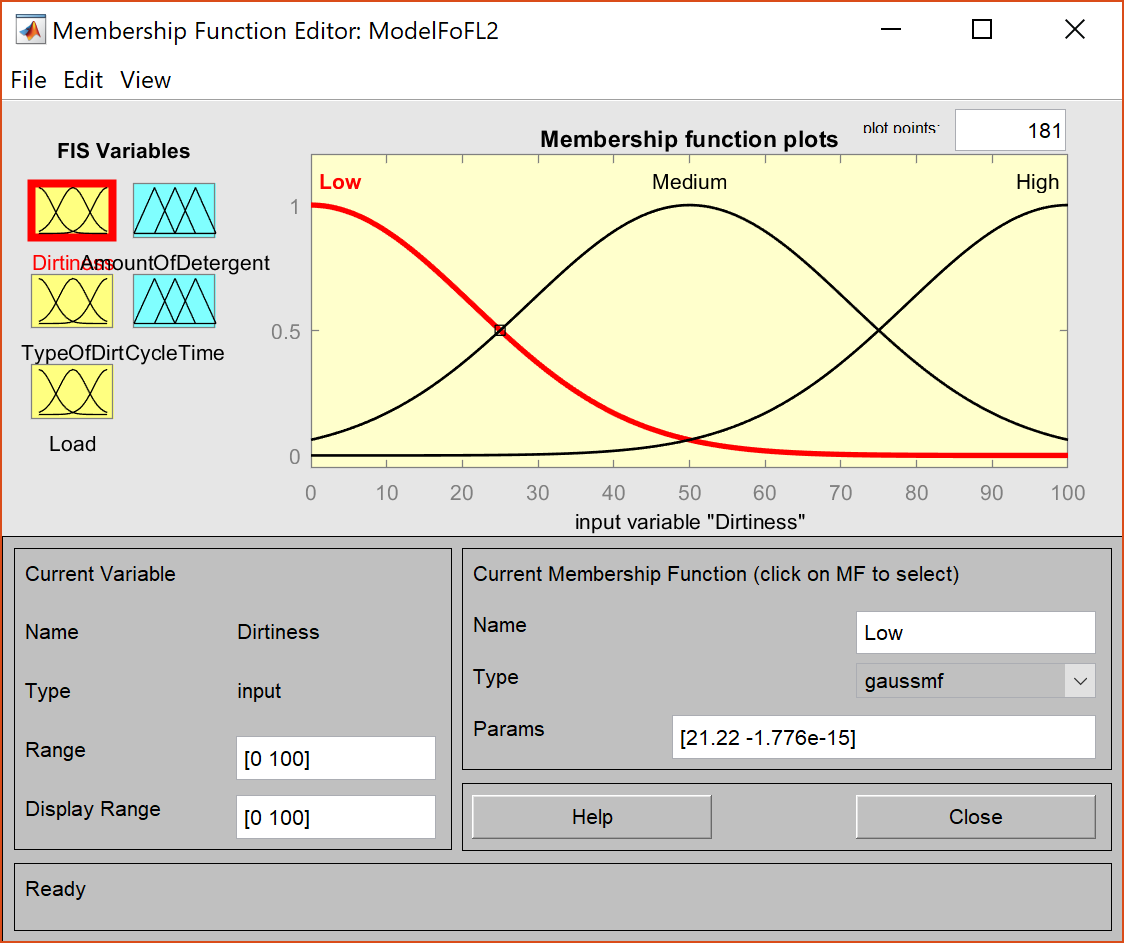
\includegraphics[width=.9\linewidth]{res/image3_dirtiness}
    \caption{ModelFoFL - Dirtiness Input}
    \label{fig:sub1}
  \end{subfigure}%
  \begin{subfigure}{.5\textwidth}
    \centering
    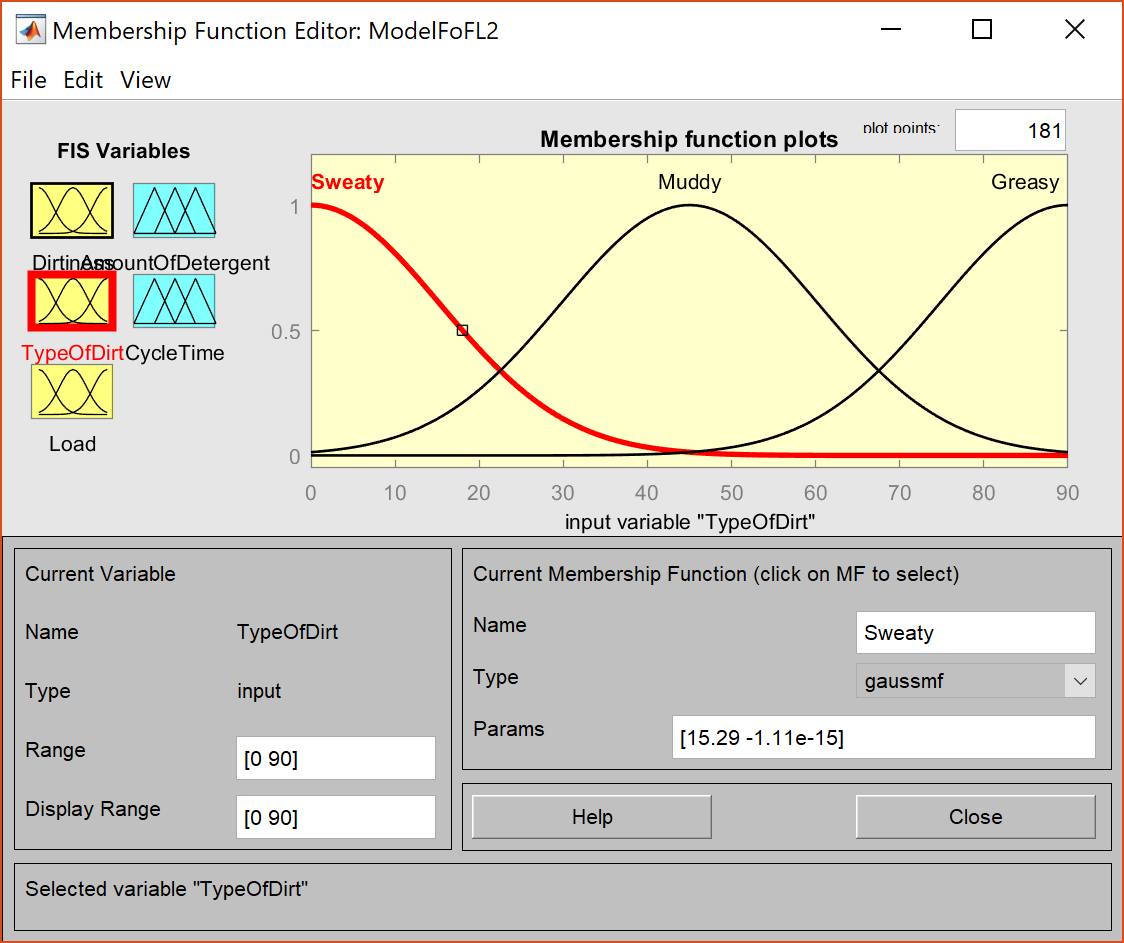
\includegraphics[width=.9\linewidth]{res/image3_dirttype}
    \caption{ModelFoFL - DirtType Input}
    \label{fig:sub2}
  \end{subfigure}
  \end{figure}

  \begin{figure}[ht!]
    \centering
    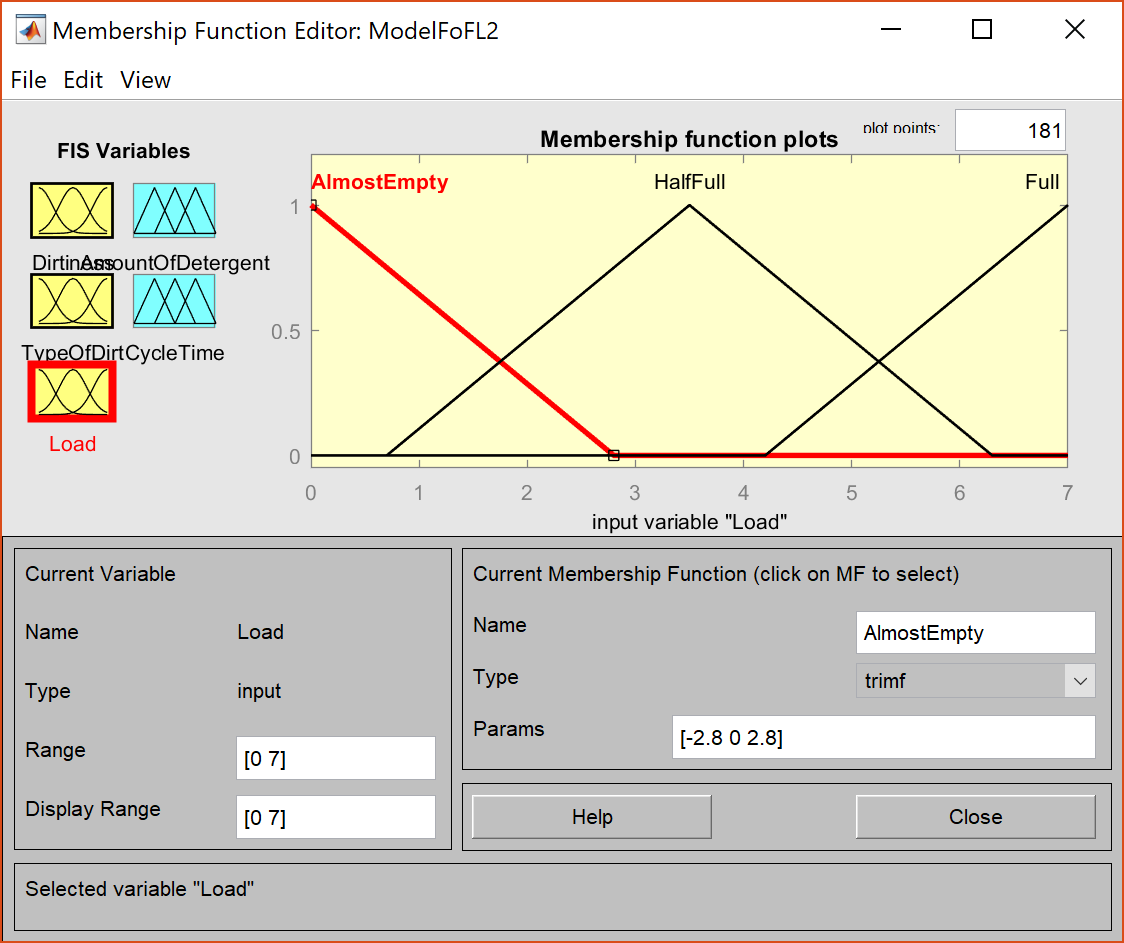
\includegraphics[width=.45\linewidth]{res/image3_load}
    \caption{ModelFoFL - Load Input}
    \label{fig:sub2}
  \end{figure}

  \begin{figure}[ht!]
  \centering
  \begin{subfigure}{.5\textwidth}
    \centering
    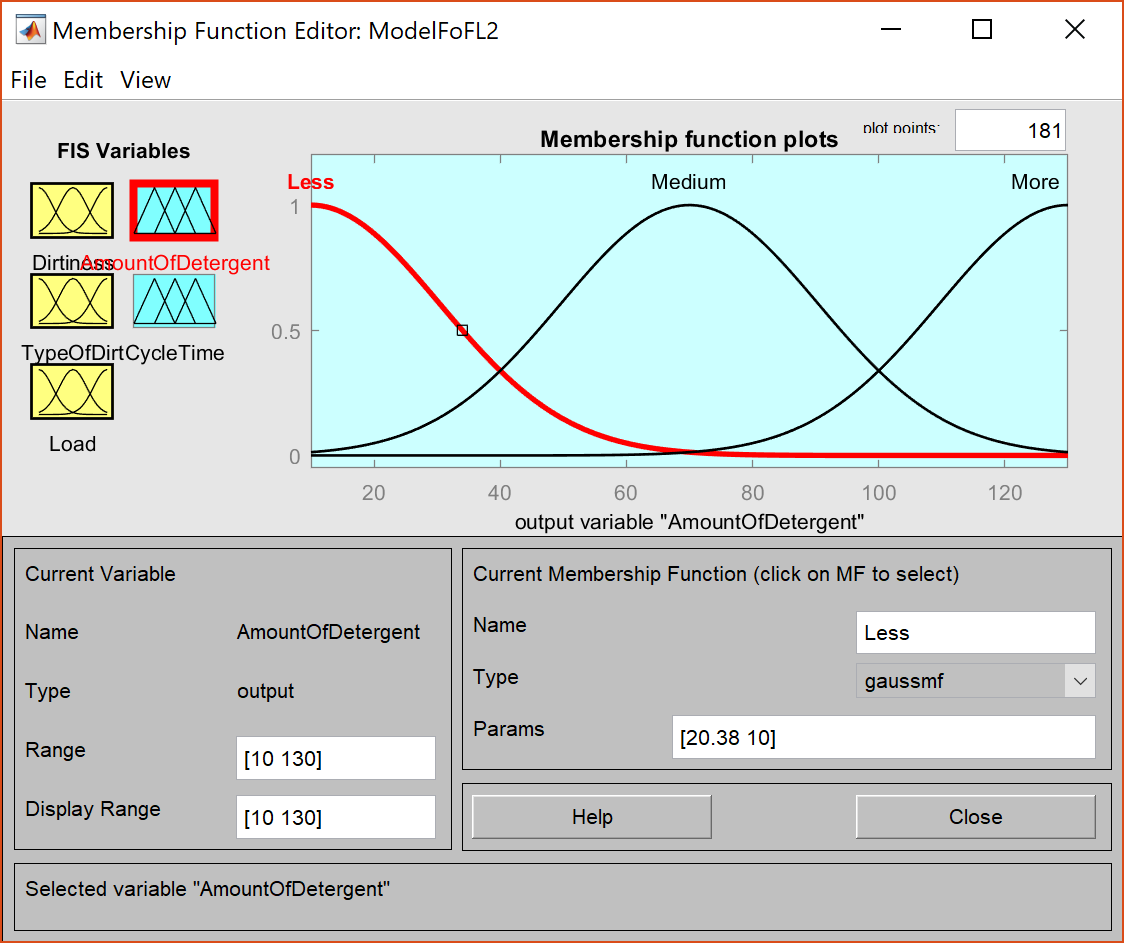
\includegraphics[width=.9\linewidth]{res/image3_detergent}
    \caption{ModelFoFL - Detergent Output}
    \label{fig:sub1}
  \end{subfigure}%
  \begin{subfigure}{.5\textwidth}
    \centering
    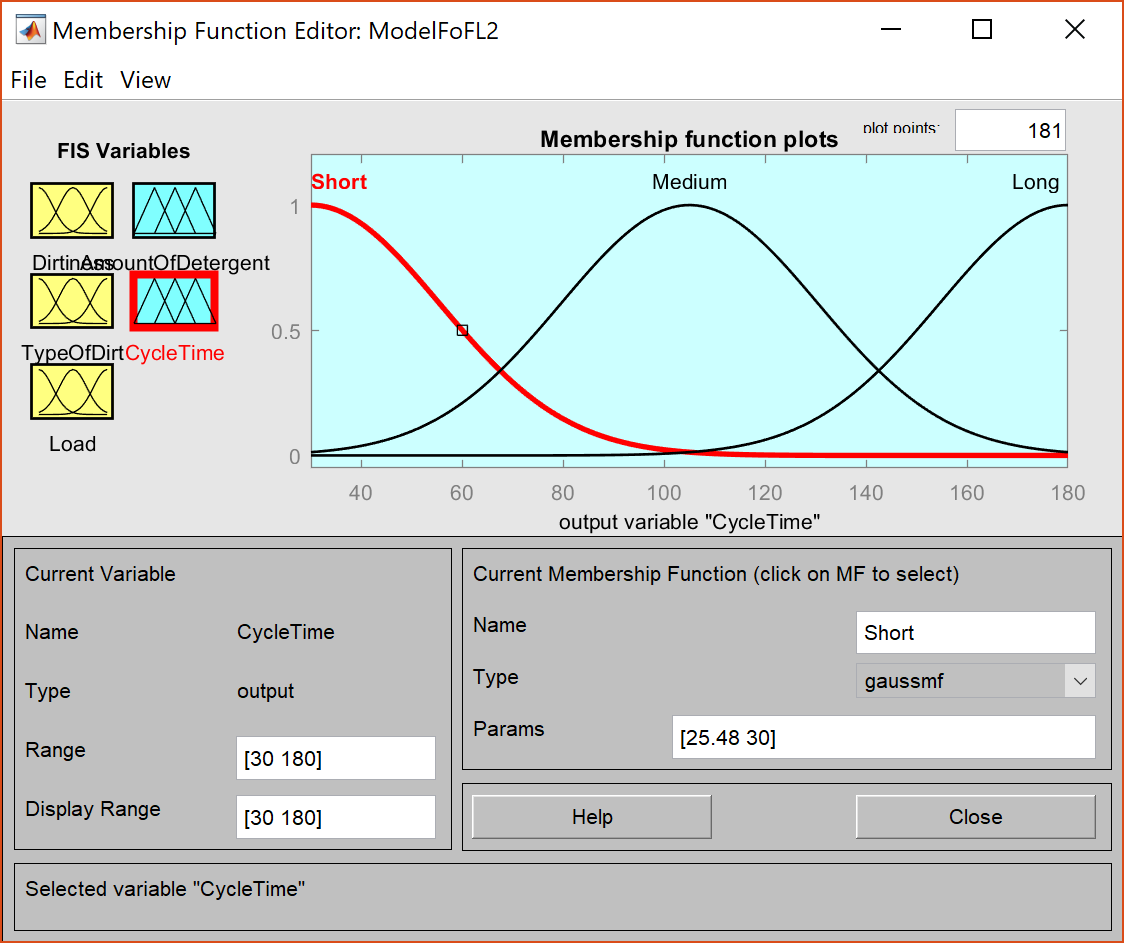
\includegraphics[width=.9\linewidth]{res/image3_cycletime}
    \caption{ModelFoFL - CycleTime Output}
    \label{fig:sub2}
  \end{subfigure}
  \end{figure}

  \begin{figure}[ht!]
  \centering
  \begin{subfigure}{.5\textwidth}
    \centering
    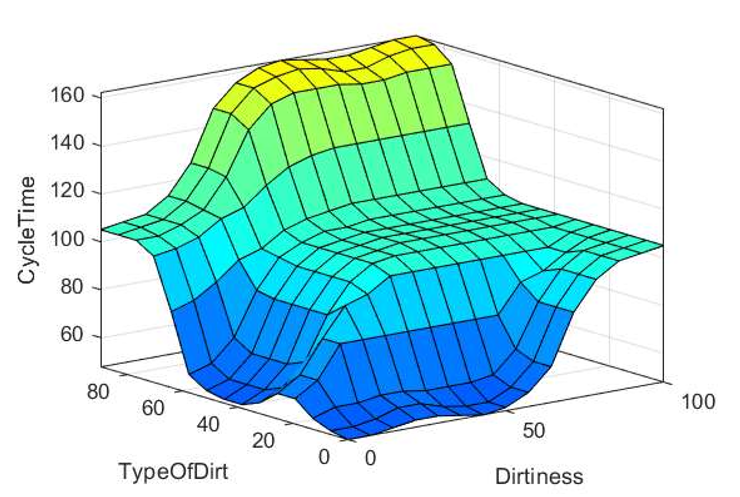
\includegraphics[width=.9\linewidth]{res/image3_surface1}
    \caption{$\langle TypeOfDirt, Dirtiness \rangle \longrightarrow CycleTime$}
    \label{fig:sub1}
  \end{subfigure}%
  \begin{subfigure}{.5\textwidth}
    \centering
    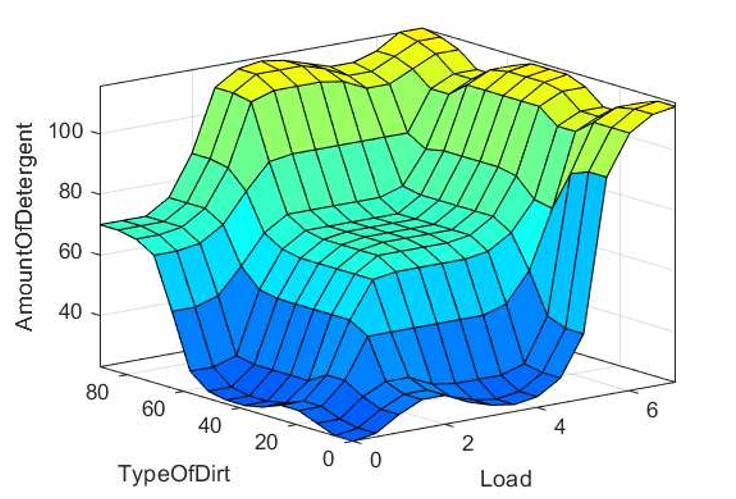
\includegraphics[width=.9\linewidth]{res/image3_surface2}
    \caption{$\langle TypeOfDirt, Load \rangle \longrightarrow
      AmountOfDetergent$}
    \label{fig:sub2}
  \end{subfigure}
  \end{figure}

  \pagebreak

  \item \textit{How did you design the membership functions for the input
  variables? Why? (Consider the number of fuzzy sets, type of fuzzy sets, the
  support and the core of the fuzzy sets)}

  I've used gaussians for the fuzzy sets that had a big range, to try and
  represent a more natural transition between fuzzy terms. For the load, I've
  used a triangular type of MF, because the load is measured in pieces of
  clothing, so the steps towards making a distinction between HalfFull or Full
  would be considered more linear.

  After playing around with the position of the MF's, adapting the support of
  the triangulars and gaussians, I reverted them back to their default
  positions because I lack the experience to tell if any improvement had been
  made.

  \pagebreak

  \item \textit{What are the rules you created? Describe your reasoning.}

  The CT model had an option to choose 'Extremely High' dirtiness,
  which gives customers the option to reduce washing time, and reduce the amount
  of detergent, lowering the cost for less dirtier clothes, and be assured that
  their clothes are completely clean having dirtier clothes, although merging
  more input options gives us more knowledge about the type of washing that
  needs to be done, and outputs can be tweaked to compensate for the lack of an
  'Extremely High' dirtiness option.

  \begin{itemize}[noitemsep]
  \item Dirtiness impacts CycleTime + Detergent
  \item Dirt type impacts CycleTime
  \item Load impacts Detergent
  \end{itemize}

  Taking the brute force way, I've created 27 rules 3*3*3 (Dirtiness * Load *
  DirtType). I've used the tables from the existing designs:

  \begin{figure}[ht!]
    \centering
    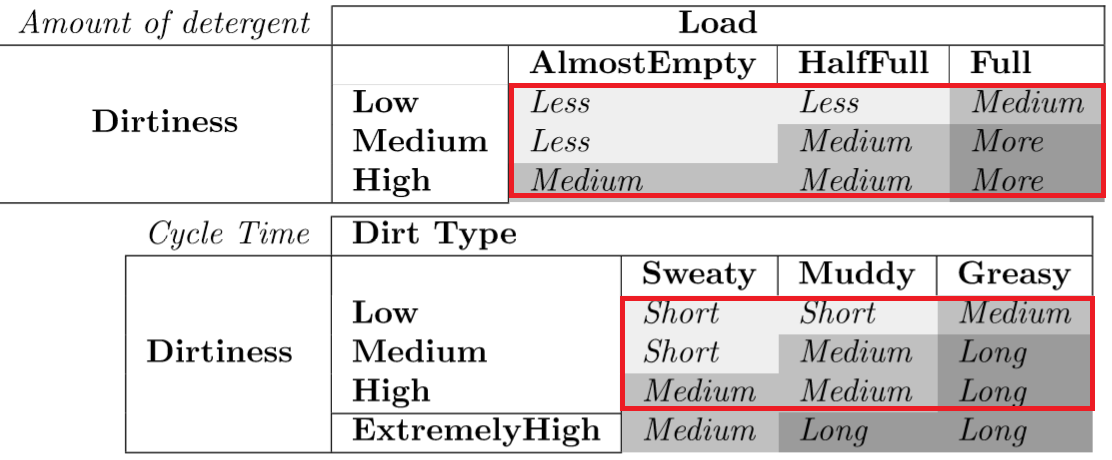
\includegraphics[width=0.9\linewidth]{res/rules_table}
    \caption{Rules Table}
  \end{figure}

  The only times that Load impacts the cycle time, and DirtType impacts the
  detergent, is when they are 'Full' and 'Greasy' respectively.

  \item What are the settings for this system? Why do you prefer these settings
  (Consider inference type, T/S-norm, aggregation, implication and
  defuzzification)

  I set all the settings to default, except for the defuzzification setting,
  because they had no impact on the surface graph. I changed the
  defuzzification setting to bisector, because it seemed to amplify the bumps
  where the cycle time and detergent would be maxed out, which would normally
  never be reached unless all the input values were exactly maxed out.

  \item By analyzing the surfaces in 2(a), discuss whether you have designed a
  washing machine that can solve the customers’ complaints.

  I would say yes, but nothing is certain until it's been tested. The wait
  times and detergent used are very low on average (of all the combinations of
  problems), keeping the costs down. As the load or type of dirt gets bigger,
  the amount of detergent increases, making sure that the dirt is tackled with
  precisely enough detergent. As the type of dirt surpasses 'Muddy', and the
  Dirtiness isn't very low, the CycleTime will be very high, to make absolutely
  sure that the wash is clean.

  \item How can you further improve your design and why?

  Tests could be run to see if the results are met. Also, the CycleTime increases in steps, which could be more like a gradient in my opinion.

\end{enumerate}


%%%%%%%%%%%%%%%%%%%%
%% Einde document %%
%%%%%%%%%%%%%%%%%%%%

\end{document}
